% =====================================================================
% Draft section — Walsh interaction vs path patching: orthogonality.
%
% Argument: Walsh coefficients (total pairwise interaction) and path
% patching (direct causal edges) measure nearly orthogonal quantities,
% showing that different discovery methods impose different selective
% pressures on the interaction structure they recover.
%
% Status: v1 first draft. Compiles with main.tex.
% Requires: booktabs, amsmath, natbib.
% =====================================================================

\subsection{Path patching and Walsh interaction are nearly orthogonal}
\label{sec:path-patching}

EAP edge scores correlate moderately with Walsh interaction coefficients
($\rho = 0.58$; Section~\ref{sec:sparse-walsh-recovery}). Path patching
isolates a narrower quantity --- the direct causal effect routed through a
specific receiver --- and might correlate more strongly with the
nonlinear interaction or might diverge. We tested the correlation on the same
20-head IOI circuit.

\paragraph{Methods.}

For each of the 176 cross-layer head pairs $(S, R)$ with
$\text{layer}(S) < \text{layer}(R)$, we computed the direct path-patch
effect: corrupt the sender's \texttt{hook\_z} with its mean across 200
IOI prompts, freeze all intermediate attention heads and MLPs to their
clean values, and let the receiver and all downstream components compute
naturally. The change in mean logit difference relative to the clean run
is the direct effect of $S$ on the output routed through $R$. Fourteen
same-layer pairs serve as a sanity check (direct effect is exactly zero
by architecture). The experiment was pre-registered before any path
patching scores were computed.

\paragraph{Result.}

Walsh interaction coefficients and path-patch direct effects are nearly
orthogonal:

\medskip

\begin{tabular}{lrr}
\toprule
 & $|w_{ij}|$ versus $|\text{PP}|$ & signed \\
\midrule
Spearman $\rho$  & $0.21$ & --- \\
Pearson $r$      & $0.13$ & $0.07$ \\
\bottomrule
\end{tabular}

\medskip

The top Walsh pair (L5H5--L8H6, $w = 0.200$) ranks 24th by direct
path-patch effect. The top path-patch edge (L10H7$\to$L11H1,
$\text{PP} = -1.96$) has a Walsh coefficient of $-0.004$, consistent
with zero interaction. The two rankings share none of their top-10 entries.

\paragraph{Mediation fraction.}

Among the 46 pairs in the top quartile of $|w_{ij}|$, 7 (15.9\%) fall
in the bottom quartile of $|\text{PP}|$ --- pairs whose Walsh interaction
is strong but whose direct causal edge is weak. These interactions are
mediated: the functional coupling between the two heads is routed through
intermediate components rather than through the direct residual-stream
path.

\paragraph{Interpretation.}

Walsh coefficients measure total interaction: how much the joint
ablation of two heads deviates from the sum of their individual
ablations, averaged over all $2^{n-2}$ backgrounds. Path patching
measures direct information flow: how much of the sender's signal
reaches the output specifically through the receiver, with all other
paths frozen. The two quantities can diverge whenever a pair interacts
primarily through a shared intermediary --- a head that reads from one
and writes to the other, or an MLP that transforms the combined signal.

Figure~\ref{fig:pp-scatter} shows the scatter: pairs cluster along both
axes independently, with no diagonal structure. The top Walsh pair
(L5H5--L8H6) and the top path-patch edge (L10H7$\to$L11H1) occupy
opposite corners.

The near-zero correlation confirms that interaction structure and
information flow are distinct properties of a circuit. A discovery method
that ranks edges by direct causal effect (path patching, ACDC) imposes a
different selective pressure from one that ranks by total interaction
(Walsh). Neither subsumes the other: path patching finds the wiring
diagram, and Walsh finds the functional couplings. The choice of method
determines which structure the circuit retains.

\begin{figure}[t]
\centering
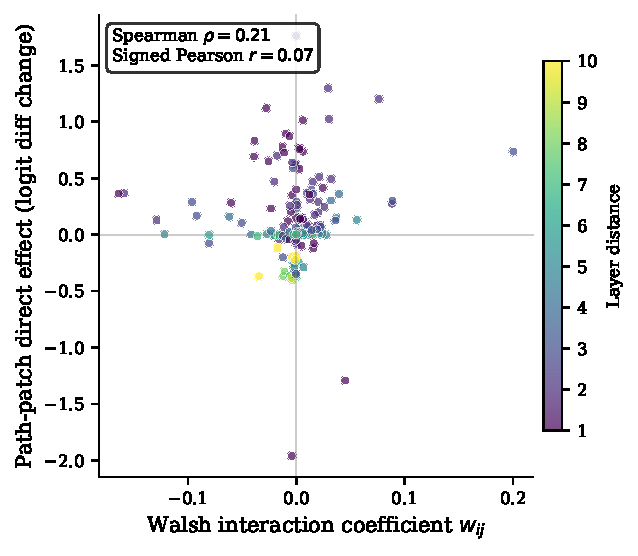
\includegraphics[width=0.65\textwidth]{figures/path_patching_scatter.pdf}
\caption{Walsh interaction coefficient versus path-patch direct effect
for 176 cross-layer head pairs in the 20-head IOI circuit. Color
indicates layer distance between sender and receiver. The two quantities
are nearly uncorrelated (signed Pearson $r = 0.07$), confirming that
functional coupling and direct information flow measure different
aspects of circuit structure.}
\label{fig:pp-scatter}
\end{figure}
